\documentclass{llncs}



%\usepackage{amssymb}
% \usepackage{amsmath}
% \usepackage{pbox}
% \usepackage{dsfont}
\setcounter{secnumdepth}{3}%%% pour que les subsubsection aient des numéros
\usepackage{paralist}
\usepackage{graphicx}
\usepackage{tikz}
\usepackage{xcolor}
\setlength\parindent{0pt}
\usepackage[colorinlistoftodos,prependcaption]{todonotes}
\usepackage{thmtools}
\usepackage{lipsum}
%\declaretheorem[style=definition]{example}

%\usepackage{xcolor,float,paralist} % del
%\usepackage{amssymb}
\usepackage{amsmath}
\usepackage{hyperref}
\usepackage{caption}
\graphicspath{{figures/}}

\usepackage [T1]{fontenc}
\usepackage[style=alphabetic, maxnames=99]{biblatex}
\addbibresource{references.bib}


\usepackage{courier}            % standard fixed width font
\usepackage[scaled]{helvet} % see www.ctan.org/get/macros/latex/required/psnfss/psnfss2e.pdf
\usepackage{url}                  % format URLs
\usepackage{enumitem}      % adjust spacing in enums
\usepackage{mathpartir}

\newcommand\var[1]{\ensuremath{\mathtt{#1}}} 
\newcommand{\keyword}[1]{\textsf{#1}}


\setcounter{biburllcpenalty}{7000}
\setcounter{biburlucpenalty}{8000}

\begin{document}


% any author declaration will be ignored  when using 'plid' option (for double blind review)

\title{Safe Dynamic Memory Management in Ada and SPARK}

\maketitle
\begin{abstract}
Handling memory in a correct and efficient way is a step toward less complex, safe, and higher performing programs and architectures. However, languages used for critical software development like Ada, including formal verification with its SPARK subset, still face challenges regarding the use of pointers due to pointer aliasing. In this work, we introduce an extension to the Ada language, and to its SPARK subset, to provide pointer types (``access types'' in Ada) that provide provably safe, automatic storage management without any asynchronous garbage collection, and without explicit deallocation by the user. Because the mechanism for these safe pointers relies on a strict control of aliasing, they can be used in the SPARK subset for formal verification, which includes both analysis of flows and proof of properties. In this paper, we present the proposal that has been submitted for inclusion in the next version of Ada, as well as the ideas underlying the inclusion of these pointers in formal analyses.
\end{abstract}

%\category{D - Software}{D.3 Programming Languages}{D.3.4 Processors - Compilers}

%\terms
%Languages, Security, Experimentation

\keywords 

Compilation, Safe Pointers, Formal Verification, Memory Management


\section{Introduction}

Standard Ada supports safe use of pointers (``access types'' in Ada) via strong type checking, but safety is guaranteed only for programs where there are no explicit deallocations of pointed-to objects -- explicit deallocation is considered ``unchecked'' programming in Ada, meaning that the programmer is responsible for ensuring that the deallocation is not performed prematurely. Ada can provide automatic reclamation of the entire memory pool associated with a particular pointer type when the pointer type goes out of scope, but it does not automatically reclaim storage prior to that point. It is possible for a user to implement abstract data types that do some amount of automatic deallocation at the object level, but this requires additional programming, and typically has certain limitations. As part of its strong type checking, Ada also prevents dangling references to objects on the stack or the heap, by providing automatic compile-time checking of ``accessibility'' levels, which reflects the lifetimes of stack and heap objects.  Conversions between pointer types are restricted to ensure pointers never outlive the objects they designate. Values of a pointer type are by default initialized to null to prevent use of uninitialized pointers, and run-time checks verify that a null pointer is never dereferenced.

\smallskip
SPARK is a subset of the Ada programming language, targeted at the most safety- and security-critical applications. SPARK starts with the basic Ada features oriented toward building reliable and long-lived software. SPARK restrictions ensure that the behavior of a SPARK program is unambiguously defined, and simple enough that formal verification tools can perform an automatic assessment of conformance between a program specification and its implementation. The SPARK language and toolset for formal verification have been applied over many years to on-board aircraft systems,
control systems, cryptographic systems, and rail systems \cite{ONeill2012, McCormick2015}.

\smallskip
As a consequence of our focus in SPARK on proof automation and usability, we have forbidden the use in SPARK of programming language features that either prevent automatic proof, or make it possible only at the expense of extensive user effort in annotating the program. The lack of support for pointers in SPARK is the main example of this choice. On the one hand, SPARK supports many Ada features that can make up for the lack of pointers: by-reference parameter passing, the ability to specify the address of objects, and the support for arrays as first-class objects. On the other hand, pointers are sometimes desirable, which forces one to exclude from formal SPARK analysis the parts of a program that make use of pointers. While there are idioms that facilitate this isolation of pointers in non-SPARK parts of a program~\cite{AdaCoreThalesSPARK}, it is highly desirable to provide some level of support for pointers in SPARK.

\smallskip
In this work, we present the first step for the inclusion of a variety of pointers that support safe memory management in Ada, in a way that these pointers can be included in SPARK. As our main contribution, we show that it is possible to adapt the ideas underlying the safe support for pointers in permission-based languages like Rust \cite{Balasubramanian17} or ParaSail \todo{add ref}, to safely restrict the use of pointers in more traditional imperative languages like Ada. 



\section{A Proposal for Ownership Types in Ada}
Pointers (access types) are essential to many complex Ada data structures, but they also have significant downsides, and can create many kinds of safety and security problems.
When attempting to prove properties about a program, particularly programs with multiple threads of control, the enemy is often the unknown ``aliasing'' of names introduced by
access types and certain uses of (potentially) by-reference parameters. We say that two names may alias if they have the possibility to refer to overlapping memory regions.
By unknown aliasing of names, we mean the situation where two distinct names might refer to the same object, without the compiler being aware of that.  A rename introduces
an alias, but not an ``unknown alias'', because the compiler is fully aware of such an alias, and hence is not something we are worrying about here. However, if a global
variable is passed by reference as a parameter to a subprogram that also has visibility on the same global, the by-reference parameter and the global are now aliases within
the subprogram, and the compiler generating code for the subprogram has no way of knowing that, hence they are ``unknown aliases''.  One approach is to always assume the worst,
but that makes analyses much harder, and in some cases infeasible. Access types also introduce unknown aliasing, and in most cases, an analysis tool will not be
sure whether the aliases exist, and will again have to make worst-case assumptions, which again may make any interesting proof infeasible.
The question that emerges in this context is: Can we create a subset of access-type functionality that supports the creation of interesting data structures without bringing along
all of the problems? The notion of pointer ``ownership'' has emerged as one way to ``tame'' pointer problems, while preserving flexibility.  The goal is to allow a pattern of use
of pointers that avoids dangling references as well as storage leaks, by providing safe, immediate, automatic reclamation of storage rather than relying on unchecked deallocation,
while also not having to fall back on the time and space vagaries of garbage collection.  As a side benefit, we can also get safer use of pointers in the context of parallelism.
We propose the use of pointer Ownership, as well as some additional rules preventing ``aliasing'' between parameters, and between parameters and global variables, to provide safe,
automatic, parallelism-friendly heap storage management while allowing the flexible construction of pointer-based data structures, such as trees, linked lists, hash tables, etc.

\smallskip
Although we took inspiration from Rust and ParaSail to produce this proposal, it is also different in many ways, due to the different objectives pursued in Ada and SPARK. Firstly,
this proposal is designed to work well with existing features of Ada such as by-copy/by-reference parameter passing and exception handling: raising an exception should not lead to
memory leaks, and upon handling of a raised exception, visible objects should not be left in an inconsistent state. Secondly, this proposal relies on the existing mechanisms in Ada
for preventing access to uninitialized pointers and freed memory: uninitialized and freed pointers should be set to null so that attempts at dereferencing such pointers results in a run-time error.




\subsection{Ownership Types}
\label{sec:ownership}

In this section, we describe the \textit{Ownership} aspect, which can be specified for an access type so that there can be either one writable access path to an object
designated by an object of such an access type, or one or more read-only access paths via such access objects, but never both concurrently. This is known as
the Concurrent-Read-Exclusive-Write (CREW) access policy. The CREW policy prevents multiple access via different objects to the same memory area whenever one
of those access objects is modifying that area.

\smallskip
Ownership is a Boolean aspect, and can be specified to be True for access types and composite types.  Objects of such a type are called ownership objects.
In addition, we use the term \textit{managed objects} to refer to all ownership objects, plus objects that are reachable by following ownership access objects.
Here is the taxonomy:

\begin{compactitem}
\item Ownership objects: objects of a type with Ownership aspect True that include:
    \begin{compactitem}
\item \textit{Owning access} objects: access-to-variable objects with Ownership aspect True;
\item \textit{Observing access} objects: access-to-constant objects with Ownership aspect True;
\item \textit{Composite ownership} objects: records and arrays with Ownership aspect True;
    \end{compactitem}
\item Other managed objects: any part of a non-ownership object designated by an owning or observing access object.
\end{compactitem}

\smallskip
In the sequel, we presume that all objects in the code examples that we will present are managed objects and refer the reader to \cite{AI2017} for further details on
the Ownership aspect specification, and specific rules that apply to non-ownership managed object. Note also that the Ownership rules will be expressed in terms
of ``names'' rather than ``objects'', since objects do not really exist at compile-time, when these rules are intended to be enforced. 

\smallskip
In the next section, we will focuse on owning access objects and observing access objects, which in Ada are passed by copy, before we
consider the situation of composite ownership objects, for which we require pass-by-reference.


\subsection{Ownership for Access Objects}
\label{subsec:ownershipAccess}

To ensure safe memory management, the basic rule is that at most one object of an access type that allows updating may be used to refer to a designated object at any time.  There might be multiple access objects that designate the same object (or some part of it) at any given time, but at most one of them may be used for updating.  Only when there are no updaters available, there can be one or more access objects that provide read-only access. The manipulation of ownership access objects in the program is limited to the following three specific kinds of operations:

\begin{compactitem}
  \item \textit{Moving}: An assignment operation that leads to moving the value of one access object into another, leaving behind a null;
  \item \textit{Borrowing}: The declaration of a short-term read-write reference by copying an existing access object, borrowing its value for the lifetime of the new reference. 
  \item \textit{Observing}: The declaration of a short-term read-only reference by copying an existing access object, observing its value for the lifetime of the reference. 
\end{compactitem}

\smallskip
Given an access object, it should have one of the three possible states after any operation:

\begin{compactitem} 
  \item \textit {Unrestricted}: the object may be dereferenced and used to read or update the designated object;
  \item \textit {Observed}: the object may be used for read-only access to all or part of the designated object, or part of some object directly or indirectly reachable via a chain of owning access objects from the designated object;
  \item \textit {Borrowed}: the object's ownership has been temporarily transferred to another object,  and while in such a state the original access object is not usable for reading or updating the designated object.
\end{compactitem}


\subsubsection{Moving Access Values}
\label{sec:moving}
\ \\

The main idea of the move operation is a complete transfer of the ownership from the right hand side access-to-variable object to the left hand side object in an assignment operation.
A moved object should hence be in the unrestricted state before the assignment. However, after the assignment, it gets set to null since the newly assigned object becomes the owner
and is unrestricted, so we must ensure the original access object has no remaining access.  By setting the original access object to null, any name that starts with a dereference of
that original access object is effectively ``destroyed''. If we do not set the original access object to null, an exception might allow the old value of the variable to be used in
an unrestricted way in the exception handler, which would be bad, particularly if the designated object had been deallocated prior to raising the exception. To avoid memory leaks,
if the prior value of the moving target is different from the new one, the object is finalized and also its storage is deallocated.  

\smallskip
We consider as a move each assignment operation where the target is a variable or a return object of a named type including an \keyword{out} or \keyword{in out} parameter.
Note that assigning to part of an aggregate is also considered as a move but will not be considered in this section which is focused only on direct manipulation of access objects.
Figure \ref{fig:move_ex1} illustrates an example of ``move'' operations. Objects \var{X} and \var{Y} are access-to-variables objects of the named type \var{Int\_Ptr}. At a \var{Swap} procedure call site,
\var{X\_Param} is \textit{copied in} from its actual parameter \var{X}, which was presumably in the unrestricted state. The ownership of \var{X.all} is then passed from \var{X} to \var{X\_Param}.
That requires setting \var{X} to null until the subprogram returns (to ensure safety in the presence of an exception), at which point \var{X\_Param} is \textit{copied back} to \var{X}.
Variable \var{X} then reasserts its ownership over \var{X.all}. Similar state transitions apply for \var{Y} and \var{Y\_Param}.  At lines $\ell_4$, $\ell_6$, and $\ell_7$,
we have additional move operations, which consist of moving, respectively, the objects \var{X\_Param}, \var{Y\_Param}, and \var{Tmp}. To conclude, thanks to our move-related rules, the naive
implementation of the Swap procedure for access types is guaranteed to be alias safe in the caller when \var{Swap} is executing and inside \var{Swap} itself since the ownership is transferred
at each access-to-variable object copy. 

\begin{figure}[htb!]
\centering
   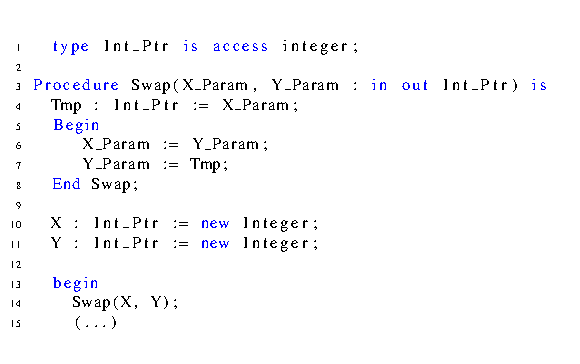
\includegraphics[]{move_ex1}
   \caption{Example for moving the ownership of an access object.}
   \label{fig:move_ex1}
\end{figure}
 

\subsubsection{Borrowing Pointer Values}
\label{sec:borrowing}
\ \\

We say that a value has been ``borrowed'' if that value has been copied into a short-lived access-to-variable managed object.
The key insight of a borrowing state is a temporary transfer of the ownership of the said borrowed object until the end of the scope of the borrower.
We effectively want the name to still designate the same object(s) until the borrower goes away. As a result, while a name that denotes a managed object
is in the borrowed state, it provides a view that allows neither reading nor updating, it is completely ``dead'' until the borrowing ends. It shall not
be used as a primary, as a prefix, as an actual parameter, nor as the target of an assignment. At the point where a static name that denotes a managed
object is borrowed, every static name that denotes the same managed object is borrowed, and every name with that static name as a prefix, is similarly borrowed.

\smallskip
We consider as borrowing some assignment operations used to \textit{initialize anonymous} stand-alone objects, \keyword{in} parameters of an access-to-variable
type, and object renaming where the renamed object is in the unrestricted state. Borrowing also affects actual parameters that are other than owning access objects
when the formal ones are of mode \keyword{out} or \keyword{in out}. We shall expand on this in Section \ref{subsec:ownershipComposite}. For now, let us consider the
code snippet of Figure \ref{fig:borrow_ex1} as a simple example for borrowing. \var{X} and \var{Y} are both access-to-variable objects. We want to swap the contents of the two
pointers using the \var{Swap\_Contents} procedure. To that end, we declare \var{X\_Param} and \var{Y\_Param} as formal parameters of mode \keyword{in}. Objects \var{X} and \var{Y} become borrowed
in the caller and in the subprogram, \var{X\_Param} and \var{Y\_Param} are the borrowers. This state gives read/write permission through these formal parameters which makes swapping
the contents safely possible. In fact, we consider this as borrowing since we want \keyword{in} parameters and stand-alone constants of an owning access type to still
provide read/write access. This is to accommodate existing practice in the use of constants of an access type to still be used to update the designated object.

\begin{figure}[htb!]
\centering
   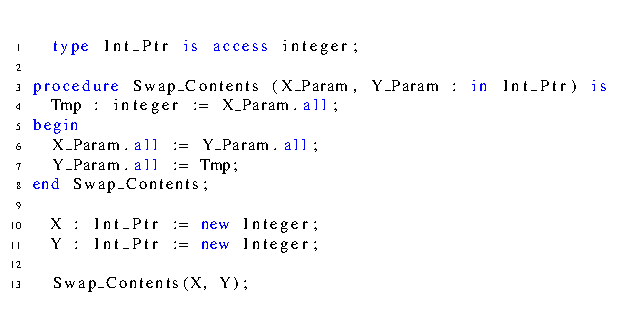
\includegraphics[]{borrow_ex1}
   \caption{Example for borrowing, \keyword{in} parameter.}
   \label{fig:borrow_ex1}
\end{figure}


\subsubsection{Observing Pointer Values}
\label{sec:observing}
\ \\

We say an access-to-variable object is ``observed'' when its value has been ``observed'', and such an object can only be used for read-only access to the designated object.
The observed state remains so until the end of the scope of the observer. While the state of a name that denotes a managed object is observed, the name shall not be moved nor
borrowed and shall not be used as the target of an assignment since we want observed objects and everything ``owned'' by them to be read only. At the point where a static name
that denotes a managed object is observed, every static name that denotes the same managed object is observed, and every name with that static name as a prefix, is similarly observed. 

\smallskip
We consider as observing some assignment operations used to \textit{initialize} anonymous stand-alone objects and parameters of an access-to-constant type.
In the code snippet of Figure \ref{fig:observe_exp}, \var{X\_Param} and \var{Y\_Param} are access-to-constant objects of an anonymous type. As the assignment of the value of \var{X} to \var{X\_Param}
as well as to \var{Y\_Param} are part of the initialization, we consider these operations as observing and assign to \var{X\_Param} and \var{Y\_Param} the read-only permission. Note that
this allows us to call the function \var{Sum} using \var{X} as a first and second parameter. The first \var{X} being observed, we still can observe it further. 

\begin{figure}[htb!]
\centering
   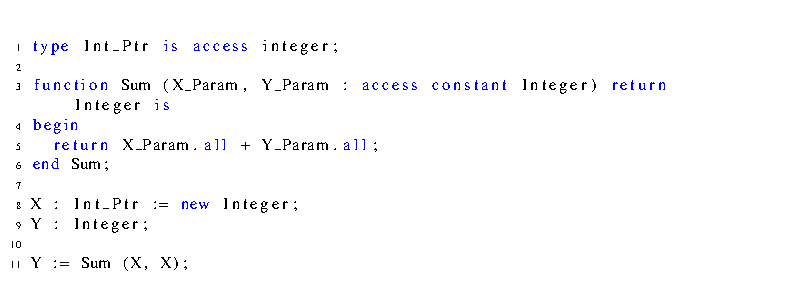
\includegraphics[]{observe_ex1}
   \caption{Example for observing a constant object.}
   \label{fig:observe_exp}
\end{figure}

\subsubsection{Preventing Read-Write Aliasing}
\label{sec:noaliasing}
\ \\

We have seen that the observing mechanism allows multiple access objects to observe the same designated object. In the scope of these objects, the designated object
cannot be written, so there is no read-write aliasing problem here.

\smallskip
We have seen that after borrowing an object, its name does not allow neither reading nor updating until the borrowing ends. For example, this prevents a call to \var{Swap\_Contents (X, X)},
as borrowing X in parameter \var{X\_Param} makes it illegal to borrow it again in parameter \var{Y\_Param}. The actual order of evaluation does not matter here, as any other order would also be illegal.

\smallskip
We have also seen that after moving an object, its value is changed to null, which prevents accessing the designated object again through the same name.
That rule in itself does not prevent a call to \var{Swap(X, X)}, as moving \var{X} in parameter \var{X\_Param} makes \var{X} null, so that it can be moved in parameter \var{Y\_Param} with value null.
Therefore, there is no read-write aliasing inside Swap. However, the actual order of evaluation matters for the functional behavior, as another order would make \var{X\_Param} null
instead. Likewise, on return from the procedure call, moving back parameter values to \var{X} may happen in two different orders, with different functional behaviors.
While obvious cases of parameter aliasing like \var{Swap(X,X)} are already illegal according to Ada 2012 rules, more complex cases that involve array indexing are neither
prevented by Ada 2012 rules nor by the rules for moving presented previously. Therefore, we have also defined a restriction \textit{No\_Parameter\_Aliasing},
in order to prevent these cases. We refer the reader to \cite{AI2017} for further details on the No\_Parameter\_Aliasing restriction.


\subsection{Extension to Composite Types} 
\label{subsec:ownershipComposite}

The rules presented previously for access objects are extended to composite ownership objects in natural ways to enforce the Concurrent-Reads-Exclusive-Write principle. 

\subsubsection{Moving Composite Values}
\label{subsubsec:movingComposite}
\ \\

Like for access objects, the main idea of the move operation is a complete transfer of the ownership from the right hand side composite object to the left hand
side object in an assignment operation. Thus, a moved object should still be in the unrestricted state before the assignment. The rules that apply for moving an
access objects are applied here to each access component of the composite type: access components of the moved objects are set to null; to avoid memory leaks, if the
prior value of the component in the moving target is different from the new one, the object is finalized and also its storage is deallocated.  

\smallskip
Like before, we consider as a move each assignment operation where the target is a variable or a return object of a composite ownership type, but this time we do not
include \keyword{out} or \keyword{in out} parameters, which are described in Section~\ref{subsubsec:borrowComposite}.

\smallskip
In the code snippet of Figure~\ref{fig:movingComposite}, \var{Rec} is a record with components of access type. The move operation occurs at line $\ell_{10}$ where \var{R} is moved
to \var{S}, which involves moving \var{R.X} into \var{S.X} and moving \var{R.Y} into \var{S.Y}. As a result, the initial objects designated by
\var{S.X} and \var{S.Y} are deallocated and \var{R.X} and \var{R.Y} end up null after the assignment. 


\begin{figure}[htb!]
\centering
   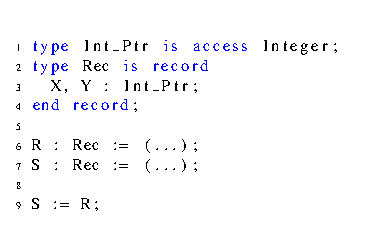
\includegraphics[]{movingComposite}
   \caption{Example for moving a composite object.}
   \label{fig:movingComposite}
\end{figure}
 
\subsubsection{Borrowing Composite Values}
\label{subsubsec:borrowComposite}
\ \\

Borrowing composite ownership objects occurs when passing such an object as \keyword{out} or \keyword{in out} parameter. This naturally applies when
such objects are passed by reference. Note the difference with \keyword{out} or \keyword{in out} parameters of an access type, which are passed by copy,
and are thus considered as moved. To avoid having two different mechanisms depending on whether a parameter is passed by-copy or by-reference, we require
that all composite ownership types are passed by reference.

\smallskip
In the code snippet of Figure~\ref{fig:borrowingComposite}, procedure \var{Swap\_Rec} has an \keyword{in out} formal parameter \var{R} of record type. At the point of
call to \var{Swap\_Rec}, the actual parameter \var{R1} becomes borrowed as formal parameter \var{R}, until returning from \var{Swap\_Rec}. Inside \var{Swap\_Rec}, the formal parameter \var{R} is initially
in unrestricted state, hence its components \var{R.X} and \var{R.Y} can be successively moved in and out through the call to \var{Swap}, and then borrowed through the call to \var{Swap\_Contents}.
Note that components of a composite type can be separately moved and borrowed, without impacting the state of other components of the same aggregate object.
The case of subcomponents is more complex, as a component is implicitly borrowed when one of its subcomponents is borrowed, and similarly in the other direction.
We refer the reader to \cite{AI2017} for further details.

\begin{figure}[htb!]
\centering
   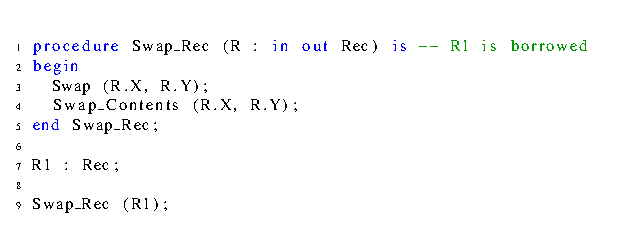
\includegraphics[]{borrowingComposite}
   \caption{Example for borrowing a composite parameter of mode \keyword{out} or \keyword{in out}.}
   \label{fig:borrowingComposite}
\end{figure}

   
\subsubsection{Observing Composite Values}
\label{subsubsec:extendingBorrowing}
\ \\

Observing composite ownership objects occurs when passing such an object as \keyword{in} parameter or initializing a constant stand-alone object of such a type. 

\smallskip
In the code snippet of Figure~\ref{fig:observingComposite}, procedure \var{Sum\_Rec} has an \keyword{in} formal parameter \var{R} of record type.
At the point of call to \var{Sum\_Rec}, the actual parameter \var{R1} becomes observed as formal parameter \var{R}, until returning from \var{Sum\_Rec}. Inside \var{Sum\_Rec},
the formal parameter \var{R} is initially in observed state, hence its components \var{R.X} and \var{R.Y} can be only be read/observed through the call to \var{Sum}.


\begin{figure}[htb!]
\centering
  \captionsetup{justification=centering,margin=0.6cm}
   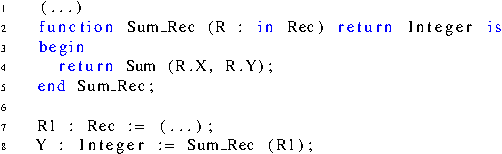
\includegraphics[]{observingComposite}
   \caption{Example for traversing a data structure with read access: Binary Search Tree Search.}
   \label{fig:observingComposite}
\end{figure}



\subsubsection{Traversing Data Structures with Local Variables}
\ \\

In the rules about borrowing access values (Section~\ref{sec:borrowing}), we said that initializing a stand-alone object of access-to-variable type corresponds to
borrowing the value. Similarly, in the rules about observing access values (Section~\ref{sec:observing}), we said that initializing a stand-alone object of
access-to-constant type correspond to observing the value. Without these special cases, such initializations would be considered as moves, and would not allow
traversing a recursive data structure in a loop with a local handle pointing to successive parts of the data structure, as every assignment to the handle would
deallocate its previous value and set the value moved to null.

\smallskip
We also special-case assignments to such stand-alone objects of anonymous access type, in order to allow traversing the data structure by changing the value of the handle.
In the borrowing case (for an access-to-variable object), the source of the assignment is restricted to a subcomponent of the object itself, which does not borrow a new object.
Doing otherwise would require data-flow analysis to determine the scope of borrowed object. In the observing case (for an access-to-constant object), the source of
the assignment is restricted to an already observed object with a compatible scope. Again, doing otherwise would require data-flow analysis to determine the scope of observed object.

\smallskip
In the code snippet of Figure~\ref{fig:maxTree}, local variable \var{Walker} is a stand-alone object of access-to-constant type that allows traversing the input binary
search tree to return the maximal value (obtained by searching for the rightmost leaf of the tree). After initializing \var{Walker} with the value of parameter \var{T},
\var{T} becomes observed, and \var{Walker} starts in the observed state (thus preventing updates to \var{T} through \var{Walker}). The data structure traversing is ensured by the instruction
of line $\ell_{16}$. 

\begin{figure}[htb!]
\centering
  \captionsetup{justification=centering,margin=0.6cm}
   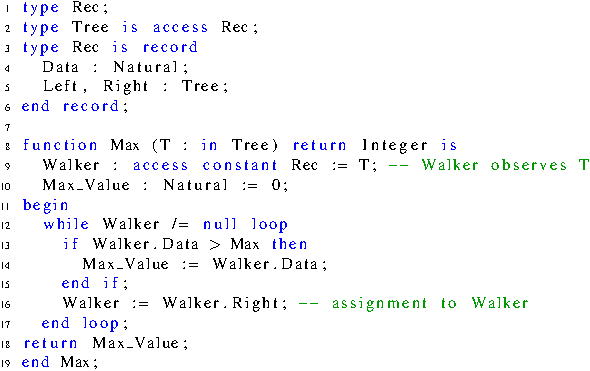
\includegraphics[]{maxTree}
   \caption{Example for traversing a data structure with read access: Binary Search Tree Search.}
   \label{fig:maxTree}
\end{figure}


In the code snippet of Figure~\ref{fig:treeInsert}, local variable \var{Walker} is a stand-alone object of access-to-variable type that allows traversing the input binary
search tree to insert the input value \var{V} at the right leaf position (obtained by searching for the leaf where this value would be stored if already present).
After initializing \var{Walker} with the value of parameter \var{T}, \var{T} becomes borrowed, and \var{Walker} starts in the unrestricted state (thus allowing updates to \var{T} through \var{Walker}).
The data structure traversing is ensured by the instruction of line $\ell_8$ and $\ell_{13}$. Insertion in the tree is performed at lines
$\ell_9$ and $\ell_{15}$.


\begin{figure}[htb!]
\centering
  \captionsetup{justification=centering,margin=0.6cm}
   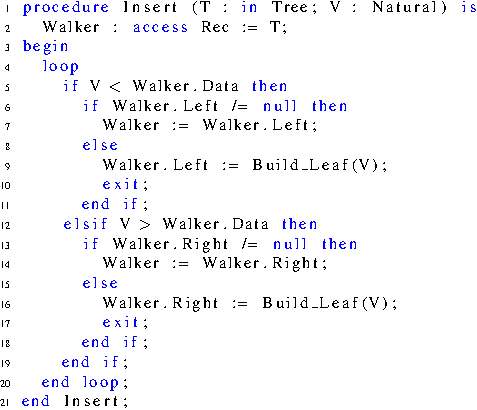
\includegraphics[]{treeInsert}
   \caption{Example for traversing a data structure with read access: Binary Search Tree Insert. \var{Build\_Leaf} is a function that creates a node such that the formal
	parameter is the value of the \var{Data} subcomponent and \var{Left} and \var{Right} subcomponents are null.}
   \label{fig:treeInsert}
\end{figure}


\section{Formal Verification with Ownership Types in SPARK}

In SPARK, an assignment to a variable cannot change the value of another visible variable. This property is essential to allow sound modular static analysis,
where each subprogram can be analyzed independently while detecting all possible violations of the kinds targeted by the analysis.

\smallskip
This is currently enforced by forbidding the use of access types in SPARK, and by restricting aliasing between parameters and global variables so that only
benign aliasing is accepted (i.e. aliasing that does not cause interference).

\smallskip
The precise rules detailed in SPARK RM 6.4.2 can be summarized as follows:

\begin{compactitem}
  \item Two output parameters should never be aliased.
  \item An input and an output parameters should not be aliased, unless the input parameter is always passed by copy.
  \item An output parameter should never be aliased with a global variable referenced by the subprogram.
  \item An input parameter should not be aliased with a global variable referenced by the subprogram, unless the input parameter is always passed by copy.
\end{compactitem}

\smallskip
To understand why aliasing matters in SPARK, consider the variation of procedure \var{Swap\_Contents} in Figure~\ref{fig:spark_ex1}. If \var{X\_Param} and \var{Y\_Param}
are not aliased, then the result of calling \var{Swap\_Contents} on actual parameters \var{X} and \var{Y} will swap their contents. If \var{X} and \var{Y} are aliased, then calling
\var{Swap\_Contents} on \var{X} and \var{X} will zero out the content of \var{X}. This is due to the assignment to \var{X\_Param.all} on line $\ell_4$.


\begin{figure}[htb!]
\centering
  \captionsetup{justification=centering,margin=0.6cm}
   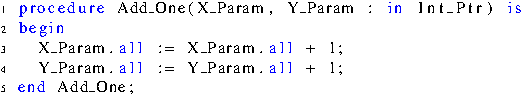
\includegraphics[]{spark_ex1}
   \caption{A variant of the \var{Swap\_Contents} procedure for which aliasing matters in SPARK.}
   \label{fig:spark_ex1}
\end{figure}

\smallskip
If SPARK ignored aliasing, it would conclude that this version of \var{Swap\_Contents} always swaps the contents of its parameters \var{X\_Param} and \var{Y\_Param}.
In particular, it could prove the following postcondition on \var{Swap\_Contents}.

\begin{figure}[htb!]
\centering
  \captionsetup{justification=centering,margin=0.6cm}
   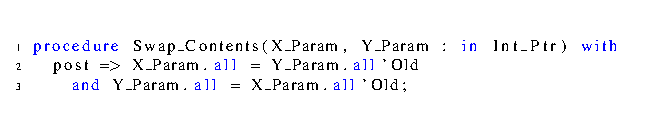
\includegraphics[]{spark_ex1_proof}
   \label{fig:spark_ex1_proof}
\end{figure}

\smallskip
Indeed, by considering that the assignment to \var{X\_Param.all} on line $\ell_4$ does not influence the value of \var{Y\_Param.all}, proof would be able to
derive that the values \var{X\_Param.all} and \var{Y\_Param.all} have been swapped. Similarly, flow analysis would derive wrong dependencies if possible aliasing is not taken into account.

\smallskip
This wrong postcondition would in turn allow to prove that a wrong assertion is satisfied in the code snippet of Figure \ref{fig:spark_ex1_exp}, while it fails at run time:

\begin{figure}[htb!]
\centering
  \captionsetup{justification=centering,margin=0.6cm}
   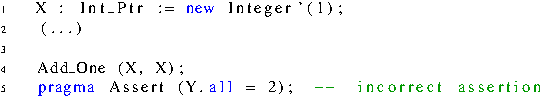
\includegraphics[]{spark_ex1_exp}
	\caption{Example for a wrong assertion due to the presence of aliasing in SPARK.}
   \label{fig:spark_ex1_exp}
\end{figure}

\smallskip
Thus, pointers cannot be treated like any other component in SPARK, in the presence of aliasing. But rules we have described for ownership objects precisely prevent
aliasing when one of the objects can be written. This is similar to the rules in SPARK for preventing aliasing between references, and this allows to treat pointers
like other components.

\smallskip
In the case of \var{Swap\_Contents}, this means that SPARK analysis will be able to conclude that the postcondition above is satisfied by the implementation of \var{Swap\_Contents}
But calls to \var{Swap\_Contents(X,X)} will be rejected both by compilation and analysis.


\section{Related Work}

\todo[inline]{Talk about Joe3 language? safeJava? “Ownership, Uniqueness, and Immutability”
A Primer on Separation Logic (and Automatic Program Verification and Analysis)
object ownership and containment
}

Permission-based programming languages generalize the issue of avoiding harmful aliasing to the more general problem of preventing harmful sharing of resources
(memory, but also network connections, files, etc.). C-like languages are mostly based on pointers and often sacrifice safety for performance purposes.
To overcome safety shortcoming and manage the storage of a pointer, C++ introduces the notion of \textit{unique pointer}. An object defined as \var{unique\_ptr}
has the ability of taking ownership of a pointer. It becomes responsible for its deletion at some point. Although enforces the language safety, the unique
pointer concept greatly limits its features by prohibiting pointer arithmetic and disabling copy assignments.

\smallskip
Separation logic~\cite{Reynolds02} is an extension of Hoare-Floyd logic that allows reasoning about pointers. In general, it is not well integrated with deductive
verification, and, in particular, is not supported by SMT provers.


\smallskip
Dafny associates each object with its \emph{dynamic frame}, the set of pointers that it owns~\cite{Leino10}. This dynamic version of Ownership is
enforced by modeling the Ownership of pointers in logic, generating verification conditions to detect violations of the single-owner model, and proving
them using SMT provers. In Spec\#, Ownership is similarly enforced by proof, to detect violations of the so-called Boogie methodology~\cite{Boogie}.

\smallskip
The inspiration for much of this work springs from the system programming in Cyclone \cite{Grossman2002} and Rust \cite{Balasubramanian17} that achieve absence of
harmful aliasing by enforcing an Ownership type system on the memory pointed-to by objects. Rust is a recent programming language targeting system
programming, with a focus on memory safety for concurrent programs.
\todo[inline]{I suggest we talk about keywords is Rust here like mut and \& which are not allowed in Ada and SPARK to highlight the difference with
Rust. Since we cannot use mut we should define rules for borrowing and its scope for instance. Since we cannot decide the by-reference passing for all object types,
we make the assumption of by-reference passing for composite types...}
Rust analysis also deals with the lifetime of allocated memory, enforcing
at the same time the lack of dangling pointer references. Pointers in Rust can never be null.\todo[inline]{How does this affect the ownership rules?}

\smallskip
The most closely related works to ours springs from Jaloyan \textit{et al.} \cite{Jaloyan18} anti-aliasing rules. In \cite{Jaloyan18}, access-to-variable objects
and composite objects with access subcomponent objects are condsidered as deep variables and their ownership states are transfered in the same way when used to call subprograms.
Actual deep parameters are considered as borrowed and the durations of borrows are only limited to duration of procedure calls.   
It turns out that this prevents traversing a linked data structure with read/write permission or even only the read permission. In this work, the distinction between stand-alone access
objects and composite ones and moving or observing composite objects instead of borrowing them has allowed us to traverse a data structure with the ability to modify something. 

\smallskip
In our work, we use a permission-based mechanism for detecting potentially harmful aliasing, in order to make the presence of pointers transparent for automated provers.
In addition, our approach does not require additional user annotations, that are required in some of the previously mentioned techniques. We thus achieve high automation
and usability, which was our goal for supporting pointers in SPARK.


\section{Conclusion}
We have presented an extension to the Ada language to provide pointer types (``access types'' in Ada) that provide provably safe, automatic
storage management without any asynchronous garbage collection, and without explicit deallocation by the user. Although we took inspiration
from Rust and ParaSail, the extension we propose is also different in many ways, in order to work well with existing features of Ada such
as by-copy/by-reference parameter passing and exception handling, and because we rely on the existing mechanisms in Ada for preventing access
to uninitialized pointers and freed memory. 

\smallskip
This extension relies on the notion of ownership, where only one access object can read and write the designated object at any given time.
Ownership of a designated object can be \textit{moved} to another object through assignment, which deallocates the object previously designated
by the target of the assignment and leaves the source of the assignment null. Ownership can also be \textit{borrowed} through a short-term read-write,
which can be either a parameter or a locally defined object. Finally, the value of a designated object can be \textit{observed} by multiple short-term
read-only references. Collectively, these mechanisms enforce a principle of Concurrent-Reads-Exclusive-Write.

\smallskip
Because the mechanism for these safe pointers relies on a strict control of aliasing, they can be used in the SPARK subset for formal verification, which
includes both analysis of flows and proof of properties. 

\smallskip
This proposal has been formalized as Ada Issue \cite{AI2017} for inclusion in the next version of Ada.

\printbibliography[title={References}]

\end{document}
